\section*{Exercise 3}

\subsection*{a)}

We now consider a function $y_2(x_1, \dots, x_5)$ which is identical to $y_1$, except all third, fourth and fifth order terms are ignored. That is:

\begin{equation}
	y_2(x_1, \dots, x_5) = b_0 + \sum_{i=1}^{5} b_i x_i + \sum_{i=1}^{4} \sum_{j=i+1}^{5} b_{ij} x_i x_j
\end{equation}

Where $b_i$, $b_{ij}$ remain unchanged. Table \ref{tab:outputs_y2} shows the result of evaluating the factorial design for this function. See part 2c) for more information.

\begin{table}[h!]
	\centering
	\begin{tabular}{cr|cr|cr|cr}
		$x_1, x_2, x_3, x_4, x_5$ &    $y_1$ & $x_1, x_2, x_3, x_4, x_5$ &    $y_1$ & $x_1, x_2, x_3, x_4, x_5$ &    $y_1$ & $x_1, x_2, x_3, x_4, x_5$ &    $y_1$ \\
		\hline
		       $-,-,-,-,-$        & $-23.56$ &        $-,-,-,-,+$        & $-32.36$ &        $-,-,-,+,-$        & $-24.67$ &        $-,-,-,+,+$        & $-31.44$ \\
		       $-,-,+,-,-$        & $-21.94$ &        $-,-,+,-,+$        & $-27.99$ &        $-,-,+,+,-$        & $-18.42$ &        $-,-,+,+,+$        & $-22.44$ \\
		       $-,+,-,-,-$        & $-28.22$ &        $-,+,-,-,+$        & $-35.65$ &        $-,+,-,+,-$        & $-27.02$ &        $-,+,-,+,+$        & $-32.41$ \\
		       $-,+,+,-,-$        & $-23.47$ &        $-,+,+,-,+$        & $-28.15$ &        $-,+,+,+,-$        & $-17.65$ &        $-,+,+,+,+$        & $-20.29$ \\
		       $+,-,-,-,-$        &  $-6.76$ &        $+,-,-,-,+$        & $-12.26$ &        $+,-,-,+,-$        &  $-2.32$ &        $+,-,-,+,+$        &  $-5.79$ \\
		       $+,-,+,-,-$        &   $2.36$ &        $+,-,+,-,+$        &  $-0.39$ &        $+,-,+,+,-$        &  $11.43$ &        $+,-,+,+,+$        &  $10.71$ \\
		       $+,+,-,-,-$        &  $-7.67$ &        $+,+,-,-,+$        &  $-11.8$ &        $+,+,-,+,-$        &  $-0.92$ &        $+,+,-,+,+$        &  $-3.01$ \\
		       $+,+,+,-,-$        &   $4.58$ &        $+,+,+,-,+$        &    $3.2$ &        $+,+,+,+,-$        &  $15.95$ &        $+,+,+,+,+$        &  $16.61$ \\
	\end{tabular}
	\caption{Outputs of the function $y2$ for all 32 possible input combinations.}
	\label{tab:outputs_y2}
\end{table}

\subsection*{b)}

The analysis of variance (ANOVA) is evaluated in the manner discussed in 2d). Only first- and second-order constributions are considered. The results can be found in Table \ref{tab:interaction_y2andknuckles}. We see that, again, the function is most sensitive to changes in $x_1$ followed by $x_3$. This is also apparent in the two-term interactions, where terms including $x_1$ and $x_3$ are larger, and $P_{13}$ has the greatest magnitude.

\begin{table}[h!]
	\centering
	\begin{tabular}{c|cc}
		Order &          1          &          2           \\
		\hline
		      & $P_{1} = 77.59\ \%$ & $P_{12} = 20.30\ \%$  \\
		      & $P_{2} = 0.04\ \%$  & $P_{13} = 37.79\ \%$ \\
		      & $P_{3} = 12.15\ \%$ & $P_{14} = 29.30\ \%$  \\
		      & $P_{4} = 4.07\ \%$  & $P_{15} = 13.96\ \%$ \\
		      & $P_{5} = 1.78\ \%$  & $P_{23} = 3.40\ \%$  \\
		      &         $-$         & $P_{24} = 1.23\ \%$  \\
		      &         $-$         & $P_{25} = 0.32\ \%$  \\
		      &         $-$         & $P_{34} = 7.57\ \%$  \\
		      &         $-$         & $P_{35} = 1.16\ \%$  \\
		      &         $-$         & $P_{45} = 0.12\ \%$  \\
		      \hline
		Total &     $95.64\ \%$     &     $115.16\ \%$     \\
	\end{tabular}
	\quad\quad\quad
	\begin{tabular}{c|cc}
		Order &          1          &          2           \\ \hline
		      & $P_{1} = 76.83\ \%$ & $P_{12} = 20.75\ \%$ \\
		      & $P_{2} = 0.12\ \%$  & $P_{13} = 37.74\ \%$ \\
		      & $P_{3} = 12.4\ \%$  & $P_{14} = 29.09\ \%$ \\
		      & $P_{4} = 4.09\ \%$  & $P_{15} = 13.99\ \%$ \\
		      & $P_{5} = 1.65\ \%$  & $P_{23} = 3.74\ \%$  \\
		      &         $-$         & $P_{24} = 1.40\ \%$  \\
		      &         $-$         & $P_{25} = 0.22\ \%$  \\
		      &         $-$         & $P_{34} = 7.68\ \%$  \\
		      &         $-$         & $P_{35} = 1.25\ \%$  \\
		      &         $-$         & $P_{45} = 0.14\ \%$  \\ \hline
		Total &     $95.08\ \%$     &     $116.00\ \%$
	\end{tabular}
	\caption{Interaction terms up to the second order in $y_2$ (left) and its stochastic counterpart (right).}
	\label{tab:interaction_y2andknuckles}
\end{table}

\subsection*{c)}

Gradient lines which represent the difference betwee $S_{ij\dots}^-$ and $S_{ij\dots}^+$ (see part 2d) can be used to visually evaluate the sensitivity of the design w.r.t. various parameter interactions. Figure \ref{fig:gradient_lines} shows the gradient lines for the first- and second-order terms in $y_2$. This figure shows, as we have already seen, that the function is most sensitive to $x_1$ followed by $x_3$. The interaction between $x_1$ and $x_3$ is also the strongest two-term interaction.

\begin{figure}[h!]
	\centering
	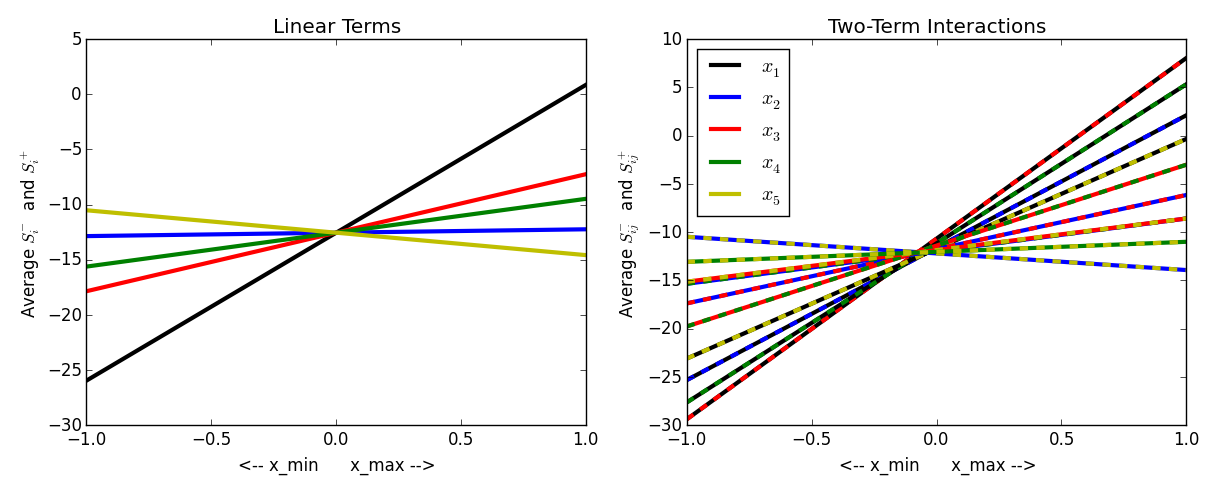
\includegraphics[width=\textwidth]{figures/gradient_lines.png}
	\caption{Gradient lines for $y_2$. A two-colored line represents the interaction between those two parameters.}
	\label{fig:gradient_lines}
\end{figure}

\subsection*{d)}

We consider the function with an added noise term which is normally distributed with mean $\mu = -0.5$ and deviation $\sigma = 1.1$. Evaluating the factorial design for this modified function yields results similar to those in Table \ref{tab:outputs_y2}, but with the described random deviation.

The ANOVA is repeated for this stochastic function. Table \ref{tab:interaction_y2andknuckles} shows an example of the interaction terms generated using it. Note that this is merely an example, and the terms are randomized. No particular pattern can be discerned from these results. Some terms are larger and some smaller than those pertaining to $y_2$, and are generally close to their original values ($\mathcal{O}(\pm 0.2\ \%)$).